\begin{problem}{1} $ $

	\begin{enumerate}
		\item 
	\begin{align*}  
 f_{XY}(x, y) &= \int f_{XYZ}(x, y, z) dz \\ 
 &= \begin{cases}
                                 \int_0^1 (x+y) dz& \text{for $0\le x, y\le 1$} \\
                                  0& \text{otherwise}
       \end{cases} \\
&= \begin{cases}
                                 x+y & \text{for $0\le x, y\le 1$} \\
                                  0& \text{otherwise}
       \end{cases}
\end{align*}
		
\item
	
	\begin{align*}  
 f_{X}(x) &= \int f_{XY}(x, y) dy \\ 
 &= \begin{cases}
                                 \int_0^1 (x+y) dy& \text{for $0\le x\le 1$} \\
                                  0& \text{otherwise}
       \end{cases} \\
&= \begin{cases}
                                 x+\frac{1}{2} & \text{for $0\le x\le 1$} \\
                                  0& \text{otherwise}
       \end{cases}
\end{align*}
	
		
		
\item First note that:
	\begin{align*}  
 f_{Z}(z) &= \int f_{XYZ}(x, y, z) dx dy \\ 
 &= \begin{cases}
                                 \int_0^1 \int_0^1 (x+y) dx dy & \text{for $0\le z \le 1$} \\
                                  0& \text{otherwise}
       \end{cases} \\
&= \begin{cases}
                                 1& \text{for $0\le z\le 1$} \\
                                  0& \text{otherwise},
       \end{cases}
\end{align*}
so that \begin{equation*}
f_{XY|Z}(x, y|z) = \frac{f_{XYZ}(x, y, z)}{f_Z(z)} = f_{XYZ}(x, y, z).
\end{equation*}



\item

\begin{equation*}
f_{XY|Z}(x, y|z) = f_{XYZ}(x, y, z) = f_{XY}(x, y)
\end{equation*}
$\implies X$ and $Y$ are independent $Z$
\end{enumerate}

\end{problem}

\begin{problem}{2} $ $

Since $X$, $Y$, $Z$ are independent, $f_{XY|Z}(x, y|1) = f_{XY}(x, y) = f_X(x)f_Y(y)$, so that:
\begin{equation*}
E[XY|Z=1] = E[XY] = E[X]E[Y] = 0,
\end{equation*}
and
\begin{equation*}
E[X^2Y^2Z^2|Z=1] = E[X^2Y^2] = E[X^2]E[Y^2] = 1.
\end{equation*}

\end{problem}

\begin{problem}{3} $ $
To solve this problem, I first state a general result for a multivariate normal.  Suppose that 

\begin{equation*}
\begin{bmatrix} \bm{X_A} \\ \bm{X_B} \end{bmatrix} \sim \mathcal N \left(\begin{bmatrix} \bm{\mu_A} \\ \bm{\mu_B }\end{bmatrix},   \left[\begin{matrix}
    \bm{\Sigma_{AA}} & \bm{\Sigma_{AB}}\\
    \bm{\Sigma_{BA}} & \bm{\Sigma_{BB}}
\end{matrix}\right] \right),
\end{equation*}
where $\bm{X_A}, \bm{\mu_A} \in \mathbb R^{m}$, $\bm{X_B}, \bm{\mu_B} \in \mathbb R^{n}$, $\bm{\Sigma_{AA}} \in \mathbb R^{m\times m}$, $\bm{\Sigma_{BB}} \in \mathbb R^{n\times n}$, $\bm{\Sigma_{AB}} \in \mathbb R^{m\times n}$ and $\bm{\Sigma_{BA}} =\bm{\Sigma_{AB}}^T $.  (Note that, here, I have written this vector equation out in the so-called ``partitioned form" for convenience.)  Then, it is not difficult to show that\footnote{for example, see: Bishop, Christopher M. Pattern Recognition and Machine Learning. Springer,
2006.}:
\begin{equation*}
\bm{X_A}|\bm{X_B} = \bm{x_B} \sim \mathcal N (\bm{\mu_A}+\bm{\Sigma_{AB}} \bm{\Sigma_{BB}}^{-1}(\bm{x_B}-\bm{\mu_{B}}), \bm{\Sigma_{AA}}-\bm{\Sigma_{AB}}\bm{\Sigma_{BB}}^{-1}\bm{\Sigma_{BA}}).
\end{equation*}

I now define the random variable, $U = Y+Z$, solve for the joint PDF of $X, Y, U$, then condition on $U$ using the formula above so that I may compute $E[XY|Y+Z=1]$.  Since $U = Y+Z$, and $Y$ and $Z$ are 2 independent $\mathcal N (1, 1)$ distributions, then $U\sim \mathcal N (2, 2)$.  Recall that for 3 marginally normal distributions, the joint distribution is:
\begin{equation*}
\begin{bmatrix} X_1 \\ X_2 \\ X_3 \end{bmatrix} \sim \mathcal N \left(\begin{bmatrix} E[X_1] \\ E[X_2]\\ E[X_3] \end{bmatrix},   \left[\begin{matrix}
    Var[X_1] & Cov[X_1, X_2]& Cov[X_1, X_3] \\
    Cov[X_2, X_1] & Var[X_2] & Cov[X_2, X_3] \\
    Cov[X_3, X_1] & Cov[X_3, X_2]& Var[X_3]
\end{matrix}\right] \right).
\end{equation*}
Thus, to solve for the joint distribution of $X, Y, U$, all that is left to do is to calculate the covariance terms involving $U$, $Cov[U, X] = Cov[Y+Z, X] = 0$ and $Cov[U, Y] = Cov[Y+Z, Y] = Var[Y]$, so the the joint distribution is:
\begin{equation*}
\begin{bmatrix} X \\ Y \\ U \end{bmatrix} \sim \mathcal N \left(\begin{bmatrix} 1 \\ 1 \\ 2 \end{bmatrix},   \left[\begin{matrix}
    1 & 0 & 0\\
    0 & 1& 1 \\
    0 & 1 & 2
\end{matrix}\right] \right).
\end{equation*}
To solve for the distribution of $X, Y|U=1$, it is not difficult to identify that, here, $\bm{\Sigma_{AA}} = I_2$ (the $2\times 2$ identity matrix), $\bm{\Sigma_{AB}}=[0, 1]^T$, $\bm{\Sigma_{BA}}=[0, 1]$, and $\bm{\Sigma_{BB}}=2$, where I identify $\bm{X_A}$ with $[X, Y]^T$ and $\bm{X_B}$ with $U$.  The mean of the conditional distribution is therefore given by
\begin{equation*}
\bm{\mu_{A|B}} = \begin{bmatrix} 1 \\ 1 \end{bmatrix}+\begin{bmatrix} 0\\1 \end{bmatrix}\frac{1}{2}(1-2)=\begin{bmatrix} 1 \\ \frac{1}{2}\end{bmatrix},
\end{equation*}
and the covariance matrix of the conditional distribution is given by:
\begin{equation*}
\bm{\Sigma_{A|B}} =\left[\begin{matrix}
    1& 0\\
    0& 1 
\end{matrix}\right] -\left[\begin{matrix}
    0 \\
    1
\end{matrix}\right] \frac{1}{2}\left[\begin{matrix}
    0,1 
\end{matrix}\right] = \left[\begin{matrix}
1 & 0\\
0& \frac{1}{2}
\end{matrix}\right].
\end{equation*}
Finally, I have the conditional distribution I desire:
\begin{equation*}
X,Y|U=1 \sim \mathcal N \left(\begin{bmatrix} 1 \\ \frac{1}{2}\end{bmatrix},   \left[\begin{matrix}
1 & 0\\
0& \frac{1}{2}
\end{matrix}\right] \right).
\end{equation*}
We would like to solve for $E[XY|U=1]$, which we can get easily from the covariance term of the above distribution: $E[XY|U=1] = Cov[X, Y|U=1]+E[X|U=1]E[Y|U=1] = 0 +(1)\cdot (1/2) = 1/2$.

\end{problem}

\begin{problem}{4} $ $
Due to the symmetry of the problem, $Y_1, Y_2, \ldots Y_n$ are all identically distributed, and thus:
\begin{equation*}
E[Y] = E[Y_1+Y_2+\ldots +Y_n] = E[Y_1]+E[Y_2]+\ldots +E[Y_n]  = nE[Y_1],
\end{equation*}
and
\begin{equation*}
Var[Y] = Var[Y_1+Y_2+\ldots +Y_n] = \sum_{i=1}^n Var [Y_i]+2 \sum_{i<j} Cov[Y_i, Y_j]  = nVar[Y_1]+2 nCov[Y_1, Y_2].
\end{equation*}
The reason there is a factor of $n$ in front of the covariance term can be seen from the matrix below (an $n=5$ example).  The summation over $i<j$ means that we can only consider pairs of $i,j$ above the diagonal (shaded cells).  Further, it is evident that $Y_i, Y_j$ pairs that are 2 or more apart are independent.  For example, $Y_2=X_2X_3$, $Y_3=X_3X_4$, $Y_4=X_4X_5$, so that $Y_2$ and $Y_3$ are not independent because they share the $X_3$ random variable, but  $Y_2$ and $Y_4$ \textit{are} independent because they share no random variables (and all the $X_i$s are independent).  Since independence $\implies$ no covariance, the only $Y_i, Y_j$ pairs that contribute to the sum are the $n-1$ terms right above the diagonal (as indicated by the spades in the figure).  We also cannot forget that the $Y_n,Y_1$ pair is not independent because they share the $X_1$ random variable (the spade in the upper right hand corner).  We thus see that there are $n$ pairs that contribute to the sum.
\definecolor{light-gray}{gray}{0.70}
\begin{center}
\bgroup
\def\arraystretch{1.5}
  \begin{tabular}{ | c | c | c | c | c | c |}
    \hline
     & $Y_1$ & $Y_2$& $Y_3$& $Y_4$& $Y_5$ \\  \hline
    $Y_1$ &\cellcolor{light-gray} &$\spadesuit$ & & &$\spadesuit$ \\ \hline
    $Y_2$ & &\cellcolor{light-gray} &$\spadesuit$ && \\ \hline
    $Y_3$ & & &\cellcolor{light-gray} & $\spadesuit$ & \\ \hline
     $Y_4$ & & & &\cellcolor{light-gray} & $\spadesuit$\\ \hline
     $Y_5$ & & & & &\cellcolor{light-gray} \\
    \hline
  \end{tabular}
  \egroup
\end{center}

It remains to compute $E[Y_1]$, $Var[Y_1]$ and $Cov[Y_1, Y_2]$.  Since $Y_1 = X_1X_2$, and $X_1, X_2 \distas{iid} Bern(p)$, the range of $Y_1$ is $\{0, 1 \}$, with probability $p^2$ of obtaining $1$ ($X_1 =1$ and $X_2 = 1$).  In other words, $Y_1\sim Bern(p^2)$, so that $E[Y_1] = p^2$ and $Var[Y_1] = p^2 (1-p^2)$.  All that is left to do is to compute the covariance:
\begin{align*}
Cov[Y_1, Y_2] &= E[Y_1Y_2]-E[Y_1]E[Y_2] \\
&= E[X_1X_2 X_2X_3]-E[X_1X_2]E[X_2X_3] \\
& = E[X_1]E[X_2^2]E[X_3]-E[X_1]E[X_2]^2E[X_3] \\
& = p\cdot p \cdot p - p\cdot p^2 \cdot p \\
& = p^3(1-p),
\end{align*}
where in the second line I have used the fact that all the $X$s are independent, and in the fourth line I have used the fact that for a $Bern(p)$ distribution, $p(1-p) = E[X^2] - p^2$. 

Thus, we have that:
\begin{equation*}
E[Y]  = np^2
\end{equation*}
and
\begin{align*}
Var[Y] &= np^2(1-p^2)+2np^3(1-p) \\
& = np^2 (3p+1)(1-p).
\end{align*}

\end{problem}

\begin{problem}{5} $ $
\begin{enumerate}
\item To solve for the expectation, note that:
\begin{align*}
E[X] &= E[X_1+X_2+\ldots+X_k] \\
&= E[X_1]+E[X_2]+\ldots+E[X_k] \\
& = \sum_{j=0}^1 j P(X_1 = j)+\sum_{j=0}^1 j P(X_2 = j)+ \ldots+\sum_{j=0}^1 j P(X_k = j) \\
& = P(X_1 = 1)+ P(X_2 = 1)+ \ldots+P(X_k = 1),
\end{align*}
where in the second line I have used the linearity of expectation.  To solve this problem, we therefore need to solve for $P(X_i = 1)$ for all $i=1, 2, \ldots, k$.

To solve for $P(X_i = 1)$, first suppose that we draw all $b+r$ balls and create a specific sequence of blues and reds.  Note that all possible sequences are equally likely to occur. To see this, as an example, suppose $r=3$ and $b=2$ and we draw the sequence $RRBRB$.  The probability that this occurs is 
\begin{equation*}
\frac{3}{3+2}\cdot \frac{3-1}{3+2-1} \cdot \frac{2}{3+2-2} \cdot \frac{3-2}{3+2-3} \cdot \frac{2-1}{3+2-4} = \frac{3!2!}{(3+2)!}.
\end{equation*}
Suppose instead we had drawn the sequence $BRRBR$.  The probability that this sequence occurs is:
\begin{equation*}
\frac{2}{3+2}\cdot \frac{3}{3+2-1} \cdot \frac{3-1}{3+2-2} \cdot \frac{2-1}{3+2-3} \cdot \frac{3-2}{3+2-4} = \frac{3!2!}{(3+2)!}.
\end{equation*}

Notice that since the probability of all possible sequences with $r=3$ and $b=2$ is simply the product of the same terms in the numerators and the same terms in the denominators, but in a different order, the probability of any possible sequence is the same product.  Thus, in general, the probability of any specific sequence occurring is $r!b!/(b+r)!$.  As a check that all possible sequences are equally as likely and the probability of each sequence is $r!b!/(b+r)!$, if we multiply this probability by the total number of distinct sequences the result should be 1.  Taking into account the indistinguishability of all red balls and all blue balls, the total number of distinct sequences is $(b+r)!/(r!b!)$.  Multiplying these values together indeed results in 1.

Now that we know that all outcomes are equally as likely and that there is a finite sample space, we can use combinatorics to find the probabilities we are after.  Let us concentrate on the $i^{th}$ draw and compute the probability that the $i^{th}$ draw is blue.  Since all sequences are equally likely to occur, to compute this probability, we need only to divide the total number of unique sequences with a blue ball in the $i^{th}$ spot by the total number of possible unique sequences.  Since all red balls are indistinguishable and all blue balls are indistinguishable, as above, the total number of unique sequences is thus $(b+r)!/(r!b!)$.  The total number of unique sequences with a blue ball in the $i^{th}$ spot is $(b+r-1)!/[r!(b-1)!]$, and therefore the probability of obtaining a blue ball in the $i^{th}$ spot, $P(X_i=1)$, is:
\begin{equation*}
P(X_i=1) = \frac{\frac{(b+r-1)!}{r!(b-1)!}}{\frac{(b+r)!}{r!b!}} = \frac{b}{b+r}.
\end{equation*}

The desired expectation value is therefore 
\begin{align*}
E[X] &= P(X_1 = 1)+ P(X_2 = 1)+ \ldots+P(X_k = 1)\\
& = \underbrace{\frac{b}{b+r}+\frac{b}{b+r}+\ldots+\frac{b}{b+r}}_\text{$k$ times} \\
& = \frac{kb}{b+r}.
\end{align*}

\item To solve for $Var[X]$, I already have $E[X]$, so I just need to solve for $E[X^2]$:
\begin{align*}
E[X^2] &= E[(X_1+X_2+\ldots+X_k)^2] \\
& = E\left[\sum_{i=1}^kX_i^2+\sum_{i, j: i \neq j} X_iX_j \right] \\
& = \sum_{i=1}^kE[X_i^2]+\sum_{i, j: i \neq j} E[X_iX_j],
\end{align*}
where in the third line I have used the linearity of expectation, and where the notation $\sum_{i, j: i \neq j}$ refers to a summation over all $i,j$ pairs ($i,j$=1, 2, \ldots, k) expect the pairs for which $i=j$ (which was accounted for in the first summation).

We have already pretty much solved for $E[X_i^2]$:
\begin{align*}
 E[X_i^2]&= \sum_{j=0}^1 j^2 P(X_i = j) \\
 &= P(X_i = 1) \\
 &= \frac{b}{b+r}, 
 \end{align*}
 so that the first summation is:
\begin{equation*}
\sum_{i=1}^kE[X_i^2] = \frac{kb}{b+r}.
\end{equation*}
The second summation is slightly more difficult.  The strategy I take is to condition on one of the random variables and to use the law of total expectation (since $X_i, X_j \in \{ 0, 1\}$, so that one of the terms will go to zero):
\begin{align*}
E[X_iX_j] &= E[X_iX_j|X_j=0]P(X_j=0)+E[X_iX_j|X_j=1]P(X_j=1) \\
&= E[X_i|X_j=1]P(X_j=1) \\
& = \left[\sum_{l=0}^1 l P(X_i =l |X_j=1)\right ]P(X_j=1) \\
& = P(X_i=1|X_j=1)P(X_j=1),
\end{align*}
I thus need to solve for $P(X_i=1|X_j=1)$, which I can do in a very similar combinatorial fashion as I did for $P(X_i=1)$.  For this probability, the total sample space is all sequences of size $k$ with $b$ blue balls and $r$ red balls, with a blue ball in the $j^{th}$ spot.  The size of the sample space is thus $(b+r-1)!/[(b-1)!r!]$.  The number of unique sequences with a blue ball in the $j^{th}$ spot and a blue ball in the $i^{th}$ spot is $(b+r-2)!/[r!(b-2)!]$, so that 
\begin{equation*}
P(X_i=1|X_j=1) = \frac{\frac{(b+r-2)!}{r!(b-2)!}}{\frac{(b+r-1)!}{(b-1)!r!}} = \frac{b-1}{b+r-1}.
\end{equation*}
Finally, the second summation is 
\begin{align*}
\sum_{i, j: i \neq j} E[X_iX_j] &= \sum_{i, j: i \neq j}P(X_i=1|X_j=1)P(X_j=1) \\
& = \sum_{i, j: i \neq j}\frac{b-1}{b+r-1}\frac{b}{b+r} \\
& = \frac{(k^2-k)(b-1)}{b+r-1}\frac{b}{b+r},
\end{align*}
so that
\begin{align*}
 E[X^2] &= \frac{kb}{b+r}+\frac{(k^2-k)(b-1)}{b+r-1}\frac{b}{b+r} \\
 &=\frac{kbr+k^2b^2-bk^2}{(b+r)(b+r-1)}.
\end{align*}

The variance is thus:
\begin{align*}
Var[X] &= E[X^2] -E[X]^2 \\
& = \frac{kbr+k^2b^2-bk^2}{(b+r)(b+r-1)}-\left(\frac{kb}{b+r}\right)^2 \\
& = \frac{kbr(b+r-k)}{(b+r)^2(b+r-1)}.
\end{align*}


\end{enumerate}
\end{problem}


\begin{problem}{6} I start by writing out the definition of the MGF:
\begin{align*}
M_X(s) & = E[e^{sX}] \\
& = \sum_{k=1}^\infty p(1-p)^{k-1} e^{sk}\\
&= \frac{p}{1-p}\left  \{\sum_{k=0}^\infty[(1-p)e^{s}]^k-1\right \},
\end{align*}
where we recognize that the summation is a geometric series, and is finite provided $(1-p)e^{s}<1$.  Using the formula for a geometric series, and simplifying, I have that:
\begin{equation*}
M_X(s) =\frac{pe^{s}}{1+(p-1)e^s},
\end{equation*}
for $s< -\ln(1-p).$


\end{problem}

\begin{problem}{7}  We can solve this problem by realizing that the $k^{th}$ derivative of the MGF evaluated at $s=0$ gives the $k^{th}$ moment of the distribution:
\begin{align*}
E[X] &= \frac{dM_X}{ds}\Big |_{s=0} \\
&= \frac{d}{ds} \left [ \frac{1}{4}+\frac{1}{2}e^s+\frac{1}{4}e^{2s} \right] \bigg |_{s=0}  \\
& = 1,
\end{align*}
\begin{align*}
E[X^2] &= \frac{d^2M_X}{ds^2}\Big |_{s=0} \\
&= \frac{d^2}{ds^2} \left [ \frac{1}{4}+\frac{1}{2}e^s+\frac{1}{4}e^{2s} \right] \bigg |_{s=0}  \\
& = \frac{3}{2}.
\end{align*}
We therefore have that $Var[X] = 3/2-1^2 = 1/2.$

\end{problem}

\begin{problem}{8}  We already know from Problem 5 in section 6.1.6 of the book that the MGF for a $\mathcal N(\mu, \sigma^2)$ distribution is $M(s) = \exp ( s\mu +\sigma^2 s^2/2 )$, and since the MGF of the sum of independent random variables is the product of the MGFs of the random variables, we have that:
\begin{align*}
M_{X+Y}(s) &= M_X(s)M_Y(s) \\
&=\exp \left(s\mu_X+\frac{\sigma_X^2 s^2}{2} \right)\exp \left(s\mu_Y+\frac{\sigma_Y^2 s^2}{2} \right) \\
& = \exp \left[s(\mu_X+\mu_Y)+\frac{s^2}{2}(\sigma_X^2+\sigma_Y^2) \right].
\end{align*}
We recognize this as the MGF of a $\mathcal N(\mu_X+\mu_Y, \sigma_X^2+\sigma_Y^2)$ distribution.  Further, by Theorem 6.1 in the book, the MGF of a random variable uniquely determines its distribution, so that indeed $X+Y \sim \mathcal N(\mu_X+\mu_Y, \sigma_X^2+ \sigma_Y^2)$.

\end{problem}


\begin{problem}{9} As a note, for the Laplace distribution, $\lambda>0$.
\begin{align*}
M_X(s) &= E[e^{sX}] \\
& = \frac{\lambda}{2}\int_{-\infty}^\infty e^{-\lambda |x|+sx}dx \\ 
&=\frac{\lambda}{2}\left [\int_{-\infty}^0e^{x(\lambda+s)}dx+ \int_0^{\infty}e^{x(s-\lambda)}dx \right]
\end{align*}
Notice that, for both integrals to be finite, we have the conditions that $\lambda +s>0$ (for the first integral) and $s- \lambda <0$ (for the second), or in other words $|s|<\lambda$.  Assuming these two conditions, the integral can easily be evaluated, and is:
\begin{equation*}
M_X(s) = \frac{\lambda^2}{\lambda^2-s^2}.
\end{equation*}

\end{problem}

\begin{problem}{10}
\begin{align*}
M_X(s) &= E[e^{sX}] \\
& = \int_0^\infty \frac{e^{sx}\lambda^\alpha x^{\alpha-1}e^{-\lambda x}}{\Gamma(\alpha)}dx \\
& = \frac{\lambda^\alpha}{\Gamma(\alpha)}\int_0^\infty x^{\alpha-1} e^{-(\lambda-s)x}dx \\
&= \frac{\lambda^\alpha}{\Gamma(\alpha)}\frac{\Gamma(\alpha)}{(\lambda-s)^\alpha}~~\mathrm{for~} s<\lambda \\
& = \left( \frac{\lambda}{\lambda-s}\right)^\alpha
\end{align*}

\end{problem}


\begin{problem}{11} For $X_i \sim Exp(\lambda)$, from Example 6.5 in the book, we have that $M_{X_i} = \lambda/(\lambda-s)$ for $s<\lambda$.  Moreover since the MGF of the sum of independent random variables is the product of the MGFs of the random variables, we have that:
\begin{align*}
M_Y(s) &= M_{X_1}(s)M_{X_2}(s) \ldots M_{X_n}(s) \\
&=\left(\frac{\lambda}{\lambda-s}\right)^n,
\end{align*}
which, from the previous problem, we notice is the MGF of a $Gamma(n, \lambda)$ random variable.  By Theorem 6.1 in the book, the MGF of a random variable uniquely determines its distribution,
so $Y\sim Gamma(n, \lambda)$.
\end{problem}

\begin{problem}{12}
By the definition of the characteristic function, we have that:
\begin{align*}
\phi_Y(\omega) &= E[e^{i \omega Y}] \\
& = E[e^{i \omega (aX+b)}] \\
&= e^{i\omega b}E[e^{i(a\omega)X}] \\
&=e^{i\omega b}\phi_X(a\omega).
\end{align*}
\end{problem}

\begin{problem}{13}$ $
\begin{enumerate}
\item  To solve for $E[\bm U]$, I first find the marginal PDFs:
	\begin{equation*}  
 f_{X}(x) = \begin{cases}
                                  \int_0^1 \frac{1}{2}(3x+y)dy & \text{for $0\le x\le 1$} \\
                                  0& \text{otherwise}
       \end{cases} \\
= \begin{cases}
                                 \frac{3}{2}x+\frac{1}{4} & \text{for $0\le x\le 1$} \\
                                  0& \text{otherwise}
       \end{cases},
\end{equation*}
and
	\begin{equation*}  
 f_{Y}(y) = \begin{cases}
                                  \int_0^1 \frac{1}{2}(3x+y)dx & \text{for $0\le y\le 1$} \\
                                  0& \text{otherwise}
       \end{cases} \\
= \begin{cases}
                                 \frac{1}{2}y+\frac{3}{4} & \text{for $0\le y\le 1$} \\
                                  0& \text{otherwise}
       \end{cases}.
\end{equation*}
Thus, $E[X] = \int_0^1x(3x/2+1/4)dx = 5/8$ and $E[Y] = \int_0^1y(y/2+3/4)dy = 13/24$, so that
\begin{equation*}
E[\bm U]  =\begin{bmatrix} E[X] \\ E[Y] \end{bmatrix}= \left[\begin{matrix}
    \frac{5}{8}  \\[6pt]
    \frac{13}{24}
\end{matrix}\right].
\end{equation*}

\item In order to solve for$\bm R_U$, I will first need to compute $E[X^2]$, $E[Y^2]$ and $E[XY]$:
\begin{equation*}
E[X^2] = \int_0^1x^2 \left(\frac{3}{2}x+\frac{1}{4} \right)dx = \frac{11}{24},
\end{equation*}
\begin{equation*}
E[Y^2] = \int_0^1y^2 \left(\frac{1}{2}y+\frac{3}{4} \right)dy = \frac{3}{8},
\end{equation*}
and
\begin{equation*}
E[XY] = \frac{1}{2}\int_0^1 \int_0^1xy (3x+y)dxdy = \frac{1}{3}.
\end{equation*}
I can now immediately write down the correlation matrix:
\begin{align*}
\bm{R_U}  &= E[\bm U \bm U^T] \\
& = \left[\begin{matrix}
    E[X^2] & E[XY] \\
    E[YX] & E[Y^2] 
\end{matrix}\right] \\
&= \left[\begin{matrix}
    \frac{11}{24} & \frac{1}{3} \\[6pt]
    \frac{1}{3} & \frac{3}{8} 
\end{matrix}\right].
\end{align*}

\item  The covariance matrix is:

\begin{align*}
\bm{C_U}  &= E[\bm U \bm U^T]-E[\bm U] E[\bm U]^T \\
& =\bm{R_U} - \left[\begin{matrix}
    E[X]^2 & E[X]E[Y] \\
    E[Y]E[X] & E[Y]^2 
\end{matrix}\right] \\
&= \left[\begin{matrix}
    \frac{11}{24} & \frac{1}{3} \\[6pt]
    \frac{1}{3} & \frac{3}{8} 
\end{matrix}\right] -
 \left[\begin{matrix}
    \left(\frac{5}{8}\right)^2 & \left(\frac{5}{8}\right) \left(\frac{13}{24}\right) \\[6pt]
    \left(\frac{13}{24}\right)\left(\frac{5}{8}\right) & \left(\frac{13}{24}\right)^2 
\end{matrix}\right]  \\
&= \left[\begin{matrix}
    \frac{13}{192} & -\frac{1}{192} \\[6pt]
    -\frac{1}{192} & \frac{47}{576}
\end{matrix}\right].
\end{align*}

\end{enumerate}
\end{problem}



\begin{problem}{14}$ $

\begin{enumerate}
\item  First note that the range of $Y$ is $[0, 1]$.  Since we know the distribution of $Y|X=x$ and the distribution of $X$, the law of total probability for PDFs will probably be useful.  Note that $f_{Y|X}(y|x) = 1/x$ for $0 \le y \le x$ and 0 otherwise, which can be written as $(1/x)\mathbbm 1 \{0 \le y \le x \}$, which will be helpful in the integral to get the bounds of integration correct:
\begin{align*}
f_Y(y)& = \int_0^1 f_{Y|X}(y|x)f_X(x)dx \\
&= \int_0^1\frac{1}{x}\mathbbm 1 \{0 \le y \le x \} dx \\
&= \int_0^1\frac{1}{x}\mathbbm 1 \{y \le x \} dx ~~\mathrm{for~}y>0\\
&=\int_y^1\frac{1}{x} dx \\
&= - \ln y,
\end{align*}
and thus
\[
  f_Y(y) =
  \begin{cases}
                                   -\ln y & \text{for $0\le y\le1$} \\
                                   0 & \text{otherwise},
  \end{cases}
\]
which I checked integrates to 1. 

Finding the PDF of $Z$ is very similar to that of finding the PDF for $Y$.  Firstly, the range of $Z$ is $[0, 2]$.  Note that in this case $f_{Z|X}(z|x) = 1/2x$ for $0 \le z \le 2x$ and 0 otherwise, which can be written as $(1/2x)\mathbbm 1 \{0 \le z \le 2x \}$, so that the integral above becomes:
\begin{align*}
f_Z(z) &= \int_0^1\frac{1}{2x}\mathbbm 1 \{z \le 2x \} dx ~~\mathrm{for~}z>0\\
&=\int_{z/2}^1\frac{1}{2x} dx \\
&= \frac{\ln 2}{2}- \frac{\ln z}{2},
\end{align*}
and thus
\[
  f_Z(z) =
  \begin{cases}
                                   \frac{\ln 2}{2}- \frac{\ln z}{2} & \text{for $0\le z\le 2$} \\
                                   0 & \text{otherwise},
  \end{cases}
\]
which I checked integrates to 1. 

\item Using the chain rule of probability, we have that:
\begin{align*}
f_{XYZ}(x, y, z) &= f_{Z|XY}(z|x, y)f_{Y|X}(y|x)f_X(x) \\
& =f_{Z|X}(z|x)f_{Y|X}(y|x)f_X(x),
\end{align*}
where in the second line I used the fact that $Z$ and $Y$ are conditionally independent given $X$.  We thus have that 
\[
  f_{XYZ}(x, y, z) =
  \begin{cases}
                                   \frac{1}{2x^2} & \text{for $0\le x \le 1 $}, 0\le y \le x, 0\le z \le 2x \\
                                   0 & \text{otherwise},
  \end{cases}
\]
which I again checked integrates to 1. 
\end{enumerate}

\end{problem}


\begin{problem}{15}$ $
\begin{enumerate}

\item As stated in the problem, we have that 
\begin{equation*}
\begin{bmatrix} X_1 \\ X_2 \end{bmatrix} \sim \mathcal N \left(\begin{bmatrix} 1 \\ 2 \end{bmatrix},   \left[\begin{matrix}
    4 & 1 \\
    1 & 1 
\end{matrix}\right] \right),
\end{equation*}
and for a bivariate normal, we know that 
\begin{equation*}
\begin{bmatrix} X_1 \\ X_2 \end{bmatrix} \sim \mathcal N \left(\begin{bmatrix} E[X_1] \\ E[X_2] \end{bmatrix},   \left[\begin{matrix}
    Var[X_1] & Cov[X_1, X_2] \\
    Cov[X_2, X_1] & Var[X_2] 
\end{matrix}\right] \right).
\end{equation*}
Thus, I have that $X_2 \sim \mathcal N(2, 1)$, so that:
\begin{align*}
P(X_2>0) &= 1-P(X_2\le 0)\\
&= 1-\Phi \left(\frac{0-2}{1} \right) \\
&= \Phi(2) \\
& \approx 0.98.
\end{align*}

\item 

\begin{align*}
\bm Y &= \bm A \bm X +\bm b \\
=& \left[\begin{matrix}
    2 & 1 \\
    -1 & 1 \\
    1 & 3  
\end{matrix}\right] \begin{bmatrix} X_1 \\ X_2 \end{bmatrix}+\begin{bmatrix} -1 \\ 0 \\1 \end{bmatrix} \\
& = \begin{bmatrix} 2X_1+X_2-1 \\ -X_1+X_2 \\X_1+3X_2+1 \end{bmatrix}
\end{align*}
$\implies$
\begin{align*}
E[\bm Y] &=  \begin{bmatrix} 2E[X_1]+E[X_2]-1 \\ -E[X_1]+E[X_2] \\E[X_1]+3E[X_2]+1 \end{bmatrix}\\
& = \begin{bmatrix} 2\cdot 1+2-1 \\ -1+2 \\1+3\cdot 2+1 \end{bmatrix} \\
& = \begin{bmatrix} 3 \\ 1 \\8 \end{bmatrix} 
\end{align*}

\item  We know that a linear combination of a multivariate Gaussian random variable is also Gaussian.  Specifically, $\bm Y$ is distributed as $\bm Y\sim \mathcal N(\bm A E[\bm X] +\bm b, \bm A \bm{C_X} \bm A^T)$, and thus the covariance matrix of $\bm Y$ is
\begin{align*}
\bm{C_Y}& =  \bm A \bm{C_X} \bm A^T \\
&=\left[\begin{matrix}
    2 & 1 \\
    -1 & 1 \\
    1 & 3  
\end{matrix}\right] \left[\begin{matrix}
    4 & 1 \\
    1 & 1
\end{matrix}\right] \left[\begin{matrix}
    2 & -1 &1 \\
    1 & 1 & 3 
\end{matrix}\right] \\
& = \left[\begin{matrix}
    21& -6 &18 \\
    -6& 3 & -13 \\
    18& -3 &19 
\end{matrix}\right].
\end{align*}
Notice that, as it should be, $\bm{C_Y}$ is symmetric.

\item As with the first part of this problem, we know that

\begin{equation*}
\begin{bmatrix} Y_1 \\Y_2 \\Y_3 \end{bmatrix} \sim \mathcal N \left(\begin{bmatrix} E[Y_1] \\ E[Y_2]  \\ E[Y_3] \end{bmatrix},   \left[\begin{matrix}
    Var[Y_1] & Cov[Y_1, Y_2] & Cov[Y_1, Y_3] \\
    Cov[Y_2, Y_1] & Var[Y_2] & Cov[Y_2, Y_3] \\
    Cov[Y_3, Y_1] & Cov[Y_3, Y_2] & Var[Y_3]
\end{matrix}\right] \right),
\end{equation*}
so that $Y_2 \sim \mathcal N(1, 3)$, and therefore:
\begin{equation*}
P(Y_2 \le 2) = \Phi \left(\frac{2-1}{\sqrt{3}} \right) \approx 0.72.
\end{equation*}

\end{enumerate}

\end{problem}

\begin{problem}{16}  To solve this problem, I first review how to ``complete the square" for matrices.  For $a \in \mathbb R$, $x, b \in \mathbb R^{m}$ and $C \in \mathbb R^{m \times m}$ (and symmetric), a quadratic of the form
\begin{equation*}
a+{\bm b}^T{\bm x} + \frac{1}{2}{\bm x}^T \bm C {\bm x}
\end{equation*}
can be factored into the form
\begin{equation*}
\frac{1}{2}({\bm x}-{\bm m})^T \bm M ({\bm x}-{\bm m})+v,
\end{equation*}
where 
\begin{equation*}
\bm M= \bm C,
\end{equation*}
\begin{equation*}
{\bm m}=-\bm C^{-1}{\bm b},
\end{equation*}
and
\begin{equation*}
v = a-\frac{1}{2} {\bm b}^T \bm C^{-1} {\bm b}.
\end{equation*}
I now explicitly write out the MGF of $\bm X$:
\begin{align*}
M_{\bm X}(s, t, r) &= E[e^{sX_1+tX_2+rX_3}] \\
& = \int_{\mathbb R^3} \exp \{ \bm s^T \bm x \}\frac{1}{(2 \pi)^{3/2} |\bm \Sigma|^{1/2}} \exp \left \{-\frac{1}{2}(\bm x-\bm \mu)^T \bm \Sigma^{-1}(\bm x-\bm \mu) \right \}d^3x\\
& =\frac{1}{(2 \pi)^{3/2} |\bm \Sigma|^{1/2}} \int_{\mathbb R^3}  \exp \left \{ -\frac{1}{2}(\bm x-\bm \mu)^T \bm \Sigma^{-1}(\bm x-\bm \mu) + \bm s^T \bm x\right \}d^3x,
\end{align*}
where $\bm x^T \equiv [x_1, x_2, x_3]$ and $\bm s^T \equiv[s, t, r]$.  To make the exponent more Gaussian looking, I now expand the exponent out and complete the square (note that since $\bm \Sigma$ is symmetric, then so too is $\bm \Sigma^{-1}$):
\begin{align*}
-\frac{1}{2}(\bm x-\bm \mu)^T \bm \Sigma^{-1}(\bm x-\bm \mu) + \bm s^T \bm x & = -\frac{1}{2}\left [ \bm x^T \bm \Sigma^{-1}\bm x -\bm x^T \bm \Sigma^{-1}\bm \mu-\bm \mu^T \bm \Sigma^{-1}\bm x  +\bm \mu^T \bm \Sigma^{-1}\bm \mu  \right ] + \bm s^T \bm x \\
 & = -\frac{1}{2} \bm x^T \bm \Sigma^{-1}\bm x +\bm \mu^T \bm \Sigma^{-1}\bm x  -\frac{1}{2} \bm \mu^T \bm \Sigma^{-1}\bm \mu + \bm s^T \bm x \\
  & = -\frac{1}{2} \bm x^T \bm \Sigma^{-1}\bm x +(\bm s^T+ \bm \mu^T \bm \Sigma^{-1})\bm x  -\frac{1}{2} \bm \mu^T \bm \Sigma^{-1}\bm \mu,
\end{align*}
where I have used the fact that $(\bm x^T \bm \Sigma^{-1}\bm \mu )^T=\bm x^T \bm \Sigma^{-1}\bm \mu$ since this is just a real number.  I can now read off $a$, $\bm b$ and $\bm C$:
\begin{equation*}
a = -\frac{1}{2} \bm \mu^T \bm \Sigma^{-1}\bm \mu,
\end{equation*}
\begin{equation*}
\bm b^T = \bm s^T+ \bm \mu^T \bm \Sigma^{-1}
\end{equation*}
and 
\begin{equation*}
\bm C = -\bm \Sigma^{-1},
\end{equation*}
so that 
\begin{equation*}
\bm b =(\bm b ^T)^T =\bm s + \bm \Sigma^{-1} \bm \mu
\end{equation*}
and 
\begin{equation*}
\bm C^{-1} = \left( -{\bm  \Sigma^{-1}}\right)^{-1}=-\bm \Sigma .
\end{equation*} 
Finally, the exponent can be re-expressed as
\begin{equation*}
-\frac{1}{2}({\bm x}-{\bm{\tilde m}})^T \bm {\tilde M }({\bm x}-{{\bm{\tilde m}}})+\tilde v,
\end{equation*}
where 
\begin{equation*}
\bm{\tilde m} = \bm \Sigma(\bm s+\bm \Sigma^{-1}\bm \mu),
\end{equation*}
\begin{equation*}
\bm{\tilde M} = \bm \Sigma^{-1}
\end{equation*}
and
\begin{align*}
\tilde v &= -\frac{1}{2} \bm \mu^T \bm \Sigma^{-1}\bm \mu +\frac{1}{2}(\bm s^T+ \bm \mu^T \bm \Sigma^{-1}) \bm \Sigma (\bm s + \bm \Sigma^{-1} \bm \mu) \\
& =\bm s^T \bm \mu +\frac{\bm s^T \bm \Sigma s}{2},
\end{align*}
so that the integral becomes:
\begin{align*}
M_{\bm X}(s, t, r) &= \exp ( \tilde v) \frac{1}{(2 \pi)^{3/2} | \bm \Sigma |^{1/2}} \int_{\mathbb R^3}  \exp \left \{ -\frac{1}{2}({\bm x}-{\bm{\tilde m}})^T \bm \Sigma^{-1}({\bm x}-{{\bm{\tilde m}}})\right \}d^3x \\
&=\exp \left ( \bm s^T \bm \mu +\frac{\bm s^T \bm \Sigma s}{2} \right ) ~~ \forall \bm s \in \mathbb R^3.
\end{align*}
I have used the fact that the integral is that of a Gaussian integrated over its entire domain, so that the integral evaluates to 1.  Note that we probably could have guessed this form of the MGF of $\bm X$, since it is the vector analogue of the 1 dimensional case: $M_X(s) = \exp \{s\mu +\sigma^2 s^2/2 \}$, as found in Problem 5 of 6.1.6 in the book.

The specified values of the mean vector and covariance matrix are:
\begin{equation*}
 \bm \mu = \left[\begin{matrix}
    1\\
    2 \\
    0
\end{matrix}\right],
\end{equation*}
and 
\begin{equation*}
\bm \Sigma = \left[\begin{matrix}
    9& 1 &-1 \\
    1& 4 & 2 \\
    -1& 2 &4
\end{matrix}\right],
\end{equation*}
and plugging in these specific values into the equation I derived above, and multiplying the matrices, I finally arrive at:
\begin{equation*}
M_{\bm X}(s, t, r) = \exp \left \{ s\left (\frac{9}{2}s+1 \right)+2t(t+1)+2r^2-rs+st+2rt \right \}.
\end{equation*}

\end{problem}

\begin{problem}{17}  Let $A_i$, $i=1, 2, 3, 4$, be the event that the $i^{th}$ component fails, so that the a failure occurs under the event $\cup_{1=i}^4A_i$.  We can thus obtain an upper limit on the event that failure occurs using the union bound:
\begin{align*}
P\left(\bigcup_{1=i}^4A_i\right) & \le \sum_{i=1}^4P(A_i) \\
& \le 4 p_f \\
&=\frac{1}{25}.
\end{align*}

\end{problem}

\begin{problem}{18} $ $
\begin{enumerate}

\item First note that for the random position of a node $(X_i, Y_i)$, $X_1, X_2, \ldots, X_n, Y_1, Y_2, \ldots, Y_n \distas{iid} Unif(0, 1)$.  Let us call the node under consideration node $j$, and let the set $\mathcal S$ be defined as $\mathcal S \equiv \{1, 2, \ldots, n \}-\{j\}$.  The probability that the node is isolated, $p_d$, is:

\begin{align*}
p_d &= P\left(\bigcap_{i \in \mathcal S}\left  [(X_j-X_i)^2+(Y_j-Y_i)^2>r^2 \right] \right) \\
& = \int_0^1 \int_0^1 P\left(\bigcap_{i \in \mathcal S}\left  [(X_i-X_j)^2+(Y_i-Y_j)^2>r^2 \right]  \Big |X_j=x_j, Y_j=y_j\right)f_{X_jYj}(x_j,y_j) dx_j dy_j \\
& = \int_0^1 \int_0^1 P\left(\bigcap_{i \in \mathcal S}\left  [(X_i-x_j)^2+(Y_i-y_j)^2>r^2 \right]  \right)f_{X_j}(x_j) f_{Y_j}(y_j) dx_j dy_j \\
& =  \int_0^1 \int_0^1 \prod_{i \in \mathcal S} P\left((X_i-x_j)^2+(Y_i-y_j)^2>r^2  \right)f_{X_j}(x_j) f_{Y_j}(y_j) dx_j dy_j \\
& =  \int_0^1 \int_0^1 \prod_{i \in \mathcal S} \left[1-P\left((X_i-x_j)^2+(Y_i-y_j)^2 \le r^2  \right)\right]f_{X_j}(x_j) f_{Y_j}(y_j) dx_j dy_j \\
& =  \int_0^1 \int_0^1 \left[1-P\left((X_1-x_j)^2+(Y_1-y_j)^2 \le r^2  \right)\right]^{n-1} f_{X_j}(x_j) f_{Y_j}(y_j) dx_j dy_j,
\end{align*}
where in the third and fourth lines I have used the fact that the random variables are independent, and in the last line, I have used symmetry.  I now must compute $P((X_1-x_j)^2+(Y_1-y_j)^2 \le r^2 )$.  If the given point $(x_j, y_j)$ is near the middle of the square (as in the upper point in Fig.~\ref{fig:prob_18}) then the probability of this event is simply the area of this circle (shaded grey region).  However, we notice that if $(x_j, y_j)$ is near the edge of the square, part of the shaded circle will get cutoff.  In fact, if $(x_j, y_j)$ is exactly at one of the corners of the unit square, for example, at $(0,0)$ as in Fig.~\ref{fig:prob_18}, then the amount of shaded area is minimized at $\pi r^2/4$.  Thus, for any given $(x_j, y_j)$, $P((X_1-x_j)^2+(Y_1-y_j)^2 \le r^2 ) \ge \pi r^2/4$.  Therefore,
\begin{align*}
p_d & \le \int_0^1 \int_0^1 \left(1-\frac{\pi r^2}{4}\right)^{n-1} f_{X_j}(x_j) f_{Y_j}(y_j) dx_j dy_j \\
&= \left(1-\frac{\pi r^2}{4}\right)^{n-1}
\end{align*}

	\begin{figure}[t]
	\centering
      		 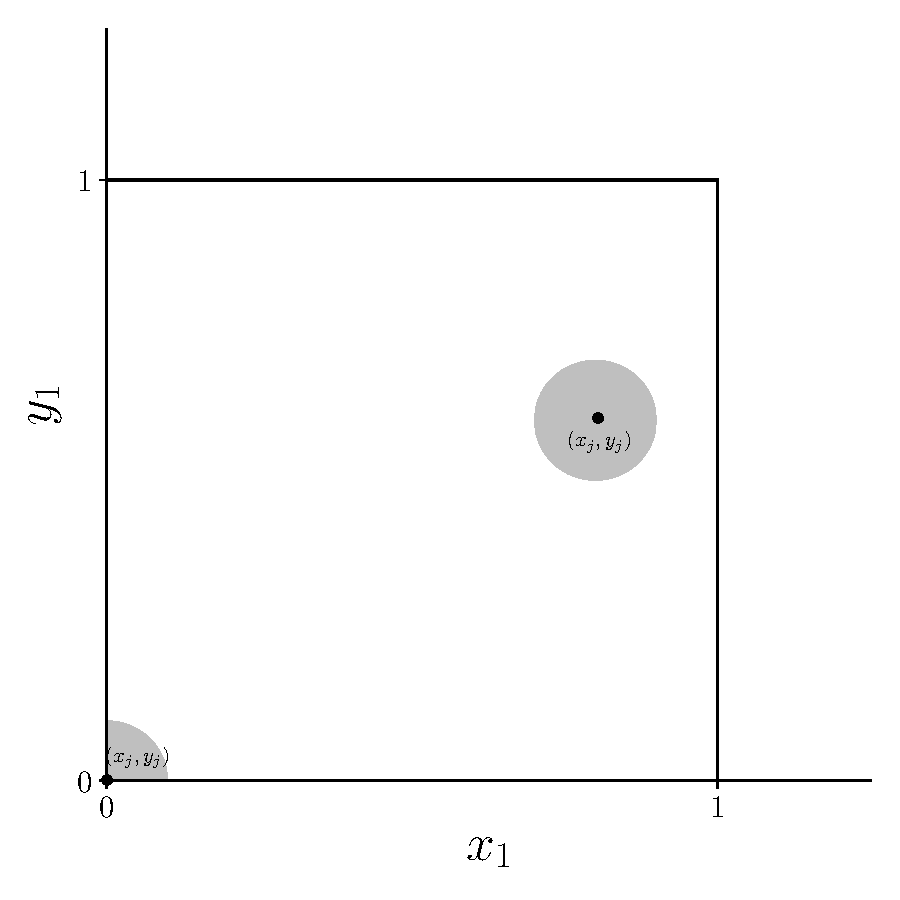
\includegraphics[totalheight=10cm]{chpt6/prob18.pdf}
  			  \caption{Two example nodes at $(x_j, y_j)$ for Problem 18.}
    			   \label{fig:prob_18}
	\end{figure}

\item Let $A_i$ be the event that the $i^{th}$ node is isolated.  Then the probability we seek is:
\begin{align*}
P\left(\bigcup_{i=1}^n A_i \right) & \le \sum_{i=1}^n P(A_i) \\
& = \sum_{i=1}^n p_d \\
& = n \left(1-\frac{\pi r^2}{4}\right)^{n-1}
\end{align*}

\end{enumerate}

\end{problem}

\begin{problem}{19}  For $X\sim Geom(p)$, $E[X] = 1/p$, so that the Markov inequality is:
\begin{equation*}
P(X \ge a) \le \frac{E[X]}{a} = \frac{1}{pa}.
\end{equation*}
The exact probability is:
\begin{align*}
P(X \ge a) &= \sum_{k=a}^\infty p(1-p)^{k-1}\\
& = \frac{p}{1-p}\left(\sum_{k=0}^\infty (1-p)^{k}-\sum_{k=0}^{a-1} (1-p)^{k} \right) \\
& = \frac{p}{1-p}\left(\frac{1}{1-(1-p)}-\frac{1-(1-p)^a}{1-(1-p)}\right) \\
&=(1-p)^{a-1}.
\end{align*}
The Markov upper bound is greater than or equal to the exact probability for $a \ge 1$ and $0<p<1$ as shown for a few values of $a$ in Fig.~\ref{fig:prob_19}

	\begin{figure}[t]
	\centering
      		 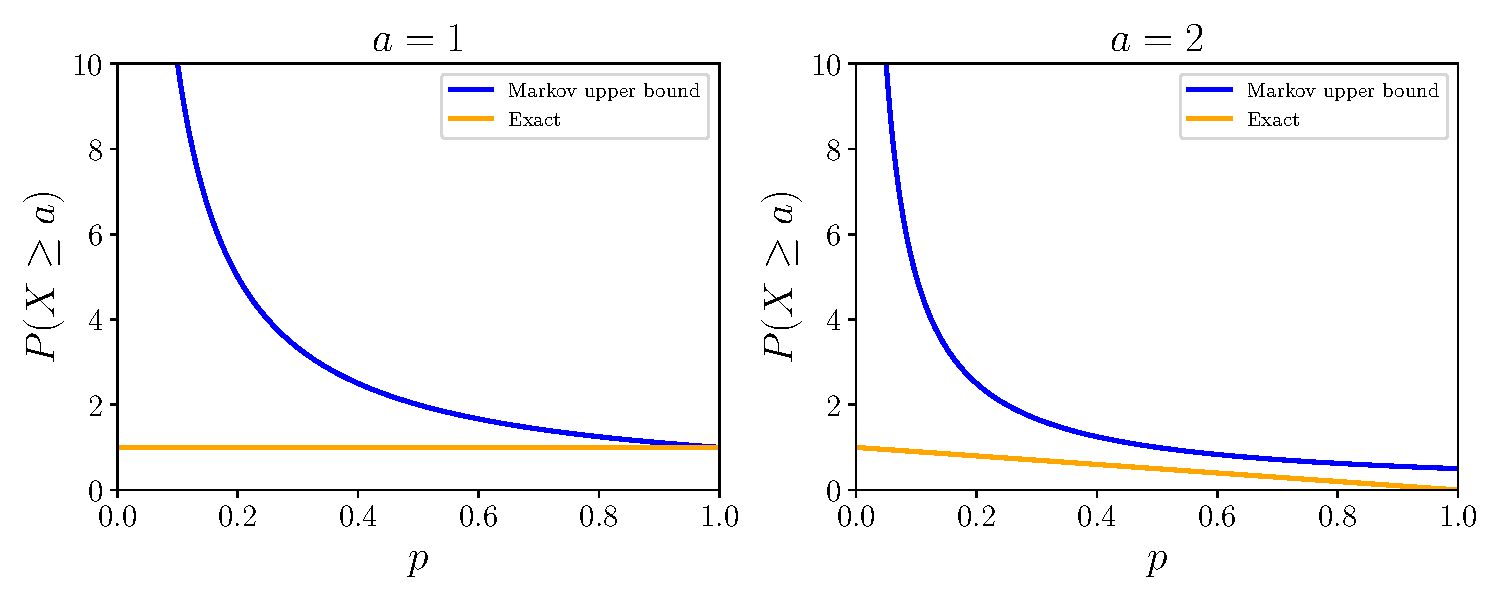
\includegraphics[totalheight=6cm]{chpt6/prob19.pdf}
  			  \caption{Comparison of Markov upper bound to exact probability for Problem 19.}
    			   \label{fig:prob_19}
	\end{figure}
\end{problem}

\begin{problem}{20}

\begin{equation*}
P(|X-E[X]|\ge b)\le \frac{Var[X]}{b^2} = \frac{1-p}{pb^2}
\end{equation*}

\end{problem}

\begin{problem}{21}
\begin{align*}
P(X \ge a) &= P\left(X+\frac{\sigma^2}{a} \ge a+\frac{\sigma^2}{a}\right) \\
&=P\left(\left(X+\frac{\sigma^2}{a}\right)^2 \ge \left (a+\frac{\sigma^2}{a} \right)^2\right) \\
& \le \frac{E\left[(X+\frac{\sigma^2}{a})^2\right]}{\left(a+\frac{\sigma^2}{a}\right)^2}~~\mathrm{Markov's~Inequality} \\
&=\frac{\sigma^2+\frac{\sigma^4}{a^2}}{a^2(1+\frac{\sigma^2}{a^2})^2} \\
& = \frac{\sigma^2}{a^2+\sigma^2}
\end{align*}

\end{problem}

\begin{problem}{22}$ $
\begin{enumerate}

\item 
\begin{align*}
P(X\le 80 \mathrm{~or~} X \ge 120) &= P(|X-100|\ge 20) \\
& = P(|X-E[X]|\ge 20) \\
& \le \frac{225}{20^2}~~ \mathrm{by~Chebyshev} \\
& = \frac{9}{16}
\end{align*}

\item
\begin{equation*}
P(X \ge 120) \le \frac{225}{225+120^2} =\frac{45}{293}
\end{equation*}

\end{enumerate}

\end{problem}

\begin{problem}{23}
We know from Problem 11 that if $X_1, X_2, \ldots, X_n\distas{iid} Exp(\lambda)$, then $Y\equiv X_1+X_2+\ldots+X_n\sim Gamma(n, \lambda)$.  The relevant Chernoff bound is given by:
\begin{equation*}
P(Y \ge a) \le \min_{s>0} \{ e^{-sa}M_X(s) \},
\end{equation*}
where, in this case the $M_X(s)$ is the MGF for a $Gamma(n, \lambda)$ distribution.  This MGF was solved for in Problem 10, and is given by
\begin{equation*}
M_X(s) = \left(\frac{\lambda}{\lambda-s}\right)^n~~\mathrm{for}~s<\lambda,
\end{equation*}
and therefore we must minimize the objective function over $0<s<\lambda$.  Let the optimal value be called $s^\star$.  I solve for $s^\star$ in the standard calculus manner by setting the derivative equal 0.  I then check to make sure that this optimal value is within the interval $(0, \lambda)$.  The derivative of the objective can be found easily with the chain rule:
\begin{equation*}
\frac{d}{ds} e^{-sa} \left(\frac{\lambda}{\lambda-s}\right)^n = -a e^{-sa} \left(\frac{\lambda}{\lambda-s}\right)^n+ne^{-sa}\left(\frac{\lambda}{\lambda-s}\right)^n\frac{1}{\lambda-s},
\end{equation*}
and setting this equal to zero and solve for $s^\star$ results in
\begin{equation*}
s^\star = \lambda - \frac{n}{a}.
\end{equation*}
As stipulated in the problem $a>n/\lambda$, which means that $n/a$ is positive and less than $\lambda$.  Thus we have that $s^\star \in (0, \lambda)$ as required.

The desired bound is therefore
\begin{align*}
P(Y\ge a) & \le e^{-s^{\star}}M_X(s^\star) \\
& = e^{-\lambda a +n}\left(\frac{\lambda a}{n} \right)^n.
\end{align*}

We can understand the behavior of this function as $n \rightarrow \infty$ by expanding the exponential in powers of $1/n$:
\begin{align*}
e^{-\lambda a +n}\left(\frac{\lambda a}{n} \right)^n &= e^{-\lambda a} \left[1 +\mathcal{O}\left(\frac{1}{n}\right) \right]\left(\frac{1}{n} \right)^n(\lambda a )^n \\
& = e^{-\lambda a} \left(\frac{\lambda a }{n} \right)^n+\mathcal{O}\left (\left(\frac{1}{n}\right)^{n+1} \right),
\end{align*}
and we thus see that the upper bound goes to 0 exponentially fast as $n$ goes to infinity.


\end{problem}

\begin{problem}{24}
Using some properties of absolute values I have that:
\begin{align*}
E[|X+Y|^{p-1}|X|] &= E[|(X+Y)^{p-1}| |X|] \\
& =E[|(X+Y)^{p-1}X|]\\
& \le E[|(X+Y)^{p-1}|^{\frac{p}{p-1}}]^{\frac{p-1}{p}}E[|X|^p]^{\frac{1}{p}}\\
&=E[|X+Y|^p]^{\frac{p-1}{p}}[|X|^p]^{\frac{1}{p}},
\end{align*}
where in the third line I have used H{\"o}lder's inequality, $E[|UV|] \le E[|U|^\alpha]^{1/\alpha}E[|V|^\beta]^{1/\beta}$, with $1<\alpha, \beta< \infty$ and $1/\alpha+1/\beta=1$, and where I have specifically chosen $\alpha=p/(p-1)$ and $\beta=p$.

Using the inequality provided in the book,
\begin{align*}
E[|X+Y|^p] & \le E[|X+Y|^{p-1}|X|] +E[|X+Y|^{p-1}|Y|] \\ 
& \le E[|X+Y|^p]^{\frac{p-1}{p}}(E[|X|^p]^{\frac{1}{p}}+E[|Y|^p]^{\frac{1}{p}}),
\end{align*}
and multiplying both sides of this equation by $E[|X+Y|^p]^{(1-p/p)}$ (which we can do without flipping the inequality sign since we know that this quantity is positive) yields the desired result:
\begin{equation*}
E[|X+Y|^p] ^{\frac{1}{p}}\le E[|X|^p]^{\frac{1}{p}}+E[|Y|^p]^{\frac{1}{p}}.
\end{equation*}

\end{problem}


\begin{problem}{25}$ $
\begin{enumerate}
\item 
\begin{equation*}
\frac{d^2}{dx^2}(x-x^3) = -6x
\end{equation*}
$\implies$ 
\[
  g^{\prime \prime}(x) =
  \begin{cases}
                                   +~\text{(convex)}& \text{for $x<0$} \\
                                   -~\text{(concave)} &  \text{for $x>0$} ,
  \end{cases}
\]
Since we know $X$ is a positive random variable, by Jensen's inequality, we have:
\begin{equation*}
E[X-X^3] \le E[X]-E[X]^3 = -990.
\end{equation*}

\item

\begin{equation*}
\frac{d^2}{dx^2}(x\ln \sqrt{x}) = \frac{1}{2x}
\end{equation*}
$\implies$ 
$ g^{\prime \prime}(x)>0$ (convex) for $x>0$
$\implies$ 
\begin{equation*}
E[X\ln \sqrt{X}] \ge E[X]\ln \sqrt{E[X]}= 10 \ln \sqrt{10}
\end{equation*}

\item  The function is a typical absolute value function, an upward v shape hitting $y=0$ at $x=2$, which is clearly convex, since a straight line drawn from any 2 points on the graph is always above the graph.  Therefore, I have that $E[|2-X|]\ge |2-E[X]| = 8.$
\end{enumerate}

\end{problem}

\begin{problem}{26} Taking the second derivative, we have that $d^2/dx^2 (x^3-6x^2) = 6x-12$.  Setting to zero and solving for $x$, I find that the second derivative is negative for $x<2$ and positive for $x>2$.  Since the range of $X$ is $(0,2)$, we have that $g(x) = x^3-6x^2$ is concave in this interval.  By Jensen's inequality, this implies that $E[Y] = E[g(X)] \le g(E[X]) = E[X]^3-6E[X]^2 = 1-6 = -5$.

\end{problem}

